\documentclass[10pt]{standalone}
\usepackage{amsmath}
\usepackage{amssymb}
\usepackage{pgf,tikz}
\usepackage{mathrsfs}
\usetikzlibrary{arrows,calc}
\pagestyle{empty}
\usepackage{siunitx}
\begin{document}
	

	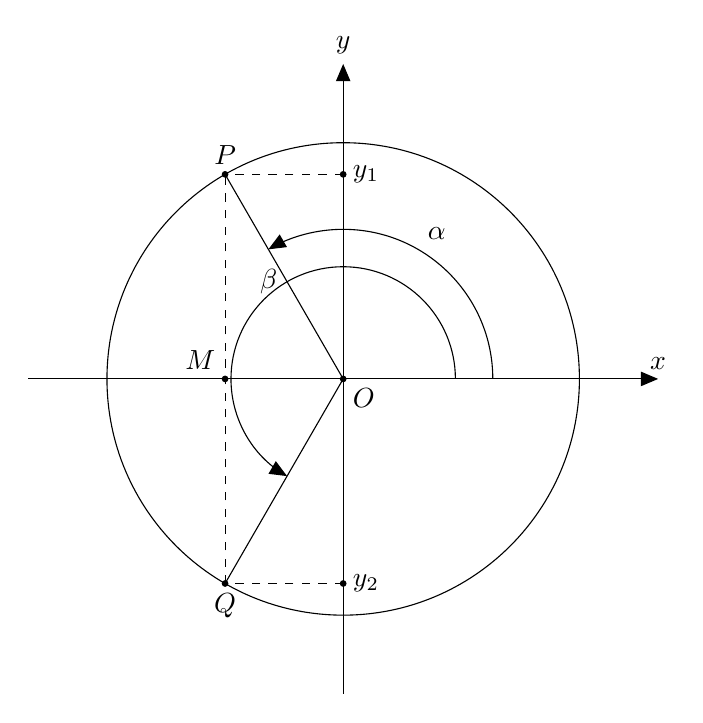
\begin{tikzpicture}[>=triangle  45]
	\tikzset{samples=600}
	\pgfmathsetmacro{\raggio}{3};
	\pgfmathsetmacro{\angolob}{60};
	\pgfmathsetmacro{\angolo}{180 -\angolob};
	\pgfmathsetmacro{\angolon}{\angolob+180};
	\pgfmathsetmacro{\y}{3};
	\pgfmathsetmacro{\xy}{4};
	\pgfmathsetmacro{\XM}{\raggio};
	\pgfmathsetmacro{\sraggio}{1.9*\raggio};
	\coordinate [label=below right:$O$] (oo)  at (0,0);
	
	\draw[->] (-\raggio-1,0) -- (\raggio+1,0) node[above] {$x$} ;
	\draw[->] (0,-\raggio-1) -- (0,\raggio+1) node[above] {$y$} ;
	\draw (oo) circle (\raggio) ;
	\coordinate[label=above:$P$] (P) at ({\raggio*cos(\angolo)},{\raggio*sin(\angolo)});
	\coordinate[label=below:$Q$] (Q) at ({\raggio*cos(\angolon)},{\raggio*sin(\angolon )});
	\coordinate [label=above left:$M$] (M) at ($((-\raggio,0)!(\angolo:\raggio)!(\raggio,0)$);
	\coordinate[label= right:$y_1$] (X1) at (0,{\raggio*sin(\angolo)});
	\coordinate[label= right:$y_2$] (X2) at (0,{\raggio*sin(\angolon)});
	\filldraw[black] (oo) circle(1pt);
	\filldraw[black] (M) circle(1pt);
	\filldraw[black] (P) circle(1pt);
	\filldraw[black] (Q) circle(1pt);
	\filldraw[black] (X1) circle(1pt);
	\filldraw[black] (X2) circle(1pt);
	\draw[dashed](Q)-- (P) ;
	\draw[dashed](X1)-- (P) ;
	\draw[dashed](X2)-- (Q) ;
	\draw[->] (\sraggio/\y,0 ) arc (0:\angolo:\sraggio/\y) ;
	\draw (\angolo/2:\sraggio/\y) node[ above right]  {$\alpha$};
	\draw[->] (\sraggio/\xy,0 ) arc (0:\angolon:\sraggio/\xy) ;
	\draw (\angolon/2:\sraggio/\xy) node[ left]  {$\beta$};
	\draw (oo)-- (P) ;
	\draw (oo)-- (Q) ;	
	
	\end{tikzpicture}
\end{document}